\section{Quotientenräume}

Seien $V,W$ $K$-Vektorräume und $U\subseteq V$ ein Untervektorraum.

\begin{definition}[affiner Unterraum]
	Ein \begriff{affiner Unterraum} von $V$ ist eine Teilmenge der Form 
	\begin{align}
		x+U:=\{x+u\mid u \in U\}\subseteq V\notag
	\end{align}
	wobei $U\subseteq V$ ein beliebiger Untervektorraum von $V$ ist und $x\in V$.
\end{definition}

\begin{lemma}
	\proplbl{3_7_2}
	Für $x,x'\in V$ sind äquivalent:
	\begin{itemize}
		\item $x+U=x'+U$
		\item $x'\in x+U$
		\item $x'-x\in U$
	\end{itemize}
\end{lemma}
\begin{proof}
	\begin{itemize}
		\item $1\Rightarrow 2$: $x'=x'+0\in x'+U=x+U$
		\item $2\Rightarrow 3$: $x'\in x+U \Rightarrow x'=x+u$ mit $u\in U\Rightarrow x'-x=u\in U$
		\item $3\Rightarrow 1$: Sei $u_0:=x'-x\in U$. Für $u\in U$ ist
		$x+u=x'-u_0+u\in x'+U$, also $x'+U\subseteq x+U$,
		$x'+u=x+u_0+u\in x+U$, also $x+U\subseteq x'+U$.
	\end{itemize}
\end{proof}

\begin{lemma}
	Sei $f\in \Hom_K(V,W)$ und $U=\Ker(f)$. Für $y\in f(V)$ ist die \begriff{Faser} $f^{-1}(y)=f^{-1}(\{y\})$ von $f$ der affine 
	Unterraum $x_0+U$ für ein beliebiges $x_0\in f^{-1}(y)$.
\end{lemma}
\begin{proof}
	$f^{-1}(y)=\{x\in V \mid f(x)=f(x_0)\}=\{x\in V \mid f(x-x_0)=0\} = \{x\in V \mid x-x_0\in U\}=x_0+U$
\end{proof}

\begin{example}
	Sind $K=\mathbb R$, $V=\mathbb R^2$, $W=\mathbb R$ und $f(x,y)=x-2y$ so sind die Fasern von $f$ die Geraden $L\subseteq 
	\mathbb R^2$ der Steigung $\frac 1 2$.
\end{example}

\begin{lemma}
	\proplbl{3_7_5}
	Seien $x_1,x'_1,x_2,x'_2\in V$ und $\lambda \in K$. Ist $x_1+U=x'_1+U$ und $x_2+U=x'_2+U$, so ist $(x_1+x_2)+U=
	(x'_1+x'_2)+U$, und $\lambda x_1+U=\lambda x'_1+U$.
\end{lemma}
\begin{proof}
	\begin{itemize}
		\item $x_1+U=x'_1+U$, $x_2+U=x'_2+U\Rightarrow x'_1-x_1,x'_2-x_2\in U\text{ \propref{3_7_2} }\Rightarrow (x'_1+x'_2)-(x_1+x_2)=(x'_1-x_1)-(x'_2-x_2)\in U
		\Rightarrow (x_1+x_2)+U=(x'_1+x'_2)+U$
		\item $x_1+U=x'_1+U\Rightarrow x'_1-x_1\in U\Rightarrow \lambda x'_1-\lambda x_1\in U\Rightarrow \lambda x'_1+U=\lambda x_1+U$
	\end{itemize}
\end{proof}

\begin{definition}[Quotientenraum]
	Der \begriff{Quotientenraum} von $V$ modulo $U$ ist die Menge der affinen Unterräume
	\begin{align}
		\qraum{V}{U}:=\{x+U\mid x\in V\}\notag
	\end{align}
	mit der Addition $(x_1+U)+(x_2+U)=(x_1+x_2)+U$ und der Multiplikation $\lambda(x+U)=\lambda x+U$. Dies ist 
	wohldefiniert nach \propref{3_7_5}.
	
	Wir definieren die Abbildung $\pi_U:V\to$ \qraum{$V$}{$U$} durch $\pi_U(x)=x+U$.
\end{definition}

\begin{proposition}
	Der Quotientenraum \qraum{$V$}{$U$} ist ein $K$-Vektorraum und $\pi_U$ ein Epimorphismus mit Kern $U$.
\end{proposition}
\begin{proof}
	\begin{itemize}
		\item $($\qraum{$V$}{$U$}$,+)$ ist eine abelsche Gruppe:
		\begin{itemize}
			\item Assoziativität un Kommutativität: überträgt sich von $(V,+)$
			\item neutrales Element: $0+U=U$
			\item inverses Element: $-(x+U)=(-x)+U$
		\end{itemize}
		\item $($\qraum{$V$}{$U$}$,+)$ ist $K$-Vektorraum: (V2) überträgt sich von $(V,+,\cdot)$
		\item $\pi_U$ surjektiv: nach Definition von \qraum{$V$}{$U$}
		\item $\pi_U$ linear: nach Definition von $+$ und $\cdot$ auf \qraum{$V$}{$U$}
		\item $\Ker(\pi_U)=\{x\in V \mid x+U=U\}=\{x\in V \mid x\in 0+U\}=U$
	\end{itemize}
\end{proof}

\begin{remark}
	Die Untervektorraum sind also genau die Kerne linearer Abbildungen! Ist $f:V\to W$ linear, so ist $\Ker(f)\subseteq V$ ein Untervektorraum. 
	Ist $U\subseteq V$ ein Untervektorraum, so ist $\pi_U:V\to$\qraum{$V$}{$U$} linear mit Kern $U$.
\end{remark}

\begin{theorem}[Homomorphiesatz]
	\proplbl{3_7_9}
	Sei $f\in \Hom_K(V,W)$ mit $U\subseteq \Ker(f)$. Dann gibt es genau eine lineare Abbildung $\tilde f:$
	\qraum{$V$}{$U$}$\to W$ mit $f=\tilde f \circ \pi_U$, d.h. es kommutiert: \\
	\begin{center}
		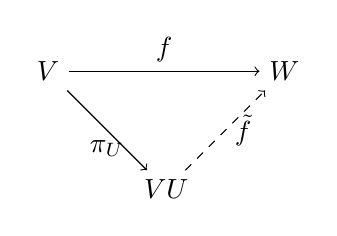
\begin{tikzpicture}
		\node (V) at (0,0) {$V$};
		\node (W) at (3,0) {$W$};
		\node (R) at (1.5,-1.5) {\qraum{$V$}{$U$}};
		\draw[->, above] (V) to node {$f$} (W);
		\draw[->, below] (V)  to node {$\pi_U$} (R);
		\draw[->, right, dashed] (R)  to node {$\tilde f$} (W);
		\end{tikzpicture}
	\end{center}
	Diese erfüllt $\Ker(\tilde f)=$\qraum{$\Ker(f)$}{U}$=\{x+U\mid x\in \Ker(f)\}\subseteq$\qraum{$V$}{$U$}.
\end{theorem}
\begin{proof}
	Ist $f=\tilde f\circ \pi_U$, so gilt $\tilde f(x+U)=\tilde f(\pi_U)=f(x)\; (*)$, somit ist $\tilde f$ dann eindeutig bestimmt. Umgekehrt 
	wird durch $(*)$ eine wohldefinierte Abbildung $\tilde f$ erklärt: Sind $x,x'\in V$ mit $x+U=x'+U$, so ist $x-x'\in U\subseteq \Ker(f)$ und 
	deshalb $f(x)=f(x')$. \\
	\begin{itemize}
		\item Linearität: Für $x,y\in V$ und $\lambda\in K$ ist $\tilde f(\lambda(x+U)+\mu(y+U))=\tilde f(\lambda\pi_U(x)+\mu\pi_U(y))=\lambda\tilde f
		(x+U)+\mu\tilde f(y+U)$.
		\item Kern: $\tilde f(x+U)=0\iff f(x)=0 \iff x\in \Ker(f)$.
	\end{itemize}
\end{proof}

\begin{conclusion}
	\proplbl{3_7_10}
	Für $f\in \Hom_K(V,W)$ ist $\Image(f)\cong $\qraum{$V$}{$\Ker(f)$}. Insbesondere gilt: Ist $f$ ein Epimorphismus, so 
	ist $W\cong $\qraum{$V$}{$\Ker(f)$}.
\end{conclusion}
\begin{proof}
	Betrachte $\tilde f:$\qraum{$V$}{$\Ker(f)$}$\to W$. Nach \propref{3_7_9} ist $\Ker(\tilde f)=$\qraum{$\Ker(f)$}{$\Ker(f)$}$=\{\Ker(f)\}$, 
	also $\tilde f$ injektiv. Nach Definition ist $\tilde f($\qraum{$V$}{$\Ker(f)$}$)=f(V)=\Image(f)$. Somit ist $\tilde f:$\qraum{$V$}
	{$\Ker(f)$}$\to \Image(f)$ ein Isomorphismus.
\end{proof}

\begin{proposition}
	\proplbl{3_7_11}
	Seien $U,U'$ Untervektorraum von $V$. Genau dann ist $V=U\oplus U'$, wenn $\pi_U|_{U'}: U'\to$\qraum{$V$}{$U$} ein Isomorphismus 
	ist.
\end{proposition}
\begin{proof}
	\begin{itemize}
		\item $\pi_U|_{U'}$ injektiv $\iff \Ker(\pi_U|_{U'})=\{0\}\iff \Ker(\pi_U)\cap U'=\{0\}\iff U\cap U'=\{0\}$
		\item $\pi_U|_{U'}$ surjektiv $\iff \forall x\in V \exists u'\in U: \pi_U(u')=\pi_U(x)\iff u'-x\in \Ker(\pi_U)=U\iff x=u+u'\iff V=U+U'$
	\end{itemize}
\end{proof}

\begin{conclusion}
	\proplbl{3_7_12}
	Ist $\dim_K(V)<\infty$, so ist $\dim_K($\qraum{$V$}{$U$}$)=\dim_K(V)-\dim_K(U)$.
\end{conclusion}
\begin{proof}
	Nach \propref{2_4_10} existiert ein lineares Komplement $U'$ zu $U$ in $V$ (d.h. $V=U\oplus U'$) und $\dim_K(U')=\dim_K(V)-\dim_K(U)$. Es gilt \qraum{$V$}
	{$U$}=$U'$.
\end{proof}

\begin{conclusion}
	\proplbl{3_7_13}
	Ist $\dim_K(V)<\infty$ und $f\in \Hom_K(V,W)$, so ist $\dim_K(V)=\dim_K(\Ker(f))+\dim_K(\Image(f))$.
\end{conclusion}
\begin{proof}
	\propref{3_7_11} und \propref{3_7_12}
\end{proof}

\begin{conclusion}
	\proplbl{3_7_14}
	Ist $\dim_K(V)<\infty$ und $f\in \End_K(V)$, so sind äquivalent:
	\begin{itemize}
		\item $f\in \Aut_K(V)$
		\item $f$ ist injektiv
		\item $f$ ist surjektiv
	\end{itemize}
\end{conclusion}
\begin{proof}
	\begin{itemize}
		\item $2\iff \dim_K(\Ker(f))=0$
		\item $3\iff \dim_K(\Image(f))=\dim_K(V)$
	\end{itemize}
\end{proof}

\begin{remark}
	Analog zu dem Quotientenräumen kann man definieren:
	\begin{itemize}
		\item Quotientengruppen \qraum{$G$}{$N$}, wobei $N$ Normalteiler von $G$ ist
		\item Quotientenringe \qraum{$R$}{$I$}, wobei $I$ ein Ideal von $R$ ist (z.B. \qraum{$\mathbb Z$}{$n\mathbb Z$})
	\end{itemize}
	Diese werden in der Vorlesung \textit{Algebra und Zahlentheorie} behandelt.
\end{remark}